% Basic Information Slide
\section{Basic Information}
\begin{frame}{Basic Information}
  \begin{itemize}
    \item \textbf{Semester:} 6th
    \item \textbf{Credits:} 4.5 ECTS (121.5 hours total)
    \begin{itemize}
      \item 39 class hours (contact hours)
      \item 39 homework hours
      \item 78 hours total workload
    \end{itemize}
    \item \textbf{Instructors:}
    \begin{itemize}
      \item Professor: Mariano Ruiz (\href{mailto:mariano.ruiz@upm.es}{mariano.ruiz@upm.es})
      \item Assistant: Cesar Gonzalez (\href{mailto:c.gonzalezb@upm.es}{c.gonzalezb@upm.es})
    \end{itemize}
  \end{itemize}
\end{frame}

% Course Language Slide

\begin{frame}{Course Language}
  \begin{itemize}
    \item \textcolor{red}{The course will be taught in \textbf{English}}.
    \item Designed for students in:
    \begin{itemize}
      \item Electronic Degree
      \item Telematics Degree
      \item Double Degree (Electronic and Telematics)
      \item Telecommunication Systems Degree
      \item International and mobility students
    \end{itemize}
    \item Communication (lectures, reports, questions, exams) will be in English.
    \item \textbf{Helpful tools:}
    \begin{itemize}
      \item Grammarly (writing assistant)
      \item ELSA Speak (pronunciation practice)
      \item Lingoes, WordReference, Google Translate (use with care)
    \end{itemize}
  \end{itemize}
\end{frame}

% Main Objectives Slide

\begin{frame}{Main Objectives}
  \begin{itemize}
    \item Identify and understand Raspberry Pi hardware and software.
    \item Build and deploy an embedded Linux distribution using Buildroot.
    \item Develop Linux applications using Eclipse (cross-compiling, linking, remote debugging).
    \item Integrate sensors into the embedded system.
    \item Understand the basic concepts and elements of the IoT model.
    \item \textbf{Bonus:} Use Git for collaborative project development.
  \end{itemize}
\end{frame}

% Requirements Slide

\begin{frame}{Requirements (not mandatory)}
  \begin{itemize}
    \item Programming in C/C++ (\href{https://web.stanford.edu/class/cs107/}{Stanford CS107}).
    \item Basic Linux command usage.
    \item Basic electronic skills (digital signals, waveforms).
    \item Office suite proficiency (documents, slides).
  \end{itemize}
\end{frame}

% Methodology Slide
\section{ECTS Methodology}
\begin{frame}{ECTS Methodology}
  \begin{columns}
    \begin{column}{0.5\textwidth}
      \begin{itemize}
        \item \textbf{Class hours (39):}
        \begin{itemize}
          \item Lectures
          \item Laboratory work
          \item Presentations (assessment)
        \end{itemize}
        \item \textbf{Student workload (39 hours):}
        \begin{itemize}
          \item Software installation
          \item Reading and comprehension
          \item Laboratory preparation
          \item Writing reports and presentations
        \end{itemize}
      \end{itemize}
    \end{column}
    \begin{column}{0.5\textwidth}
      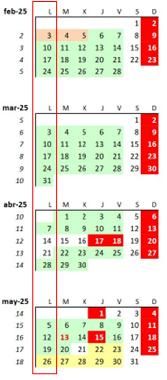
\includegraphics[height=5cm]{trainingmaterials/presentation/semester.jpg}  
    \end{column}
   \end{columns}
\end{frame}

% Course Contents Slide
\section{Course Organization}
\begin{frame}{Course Contents}
  \begin{enumerate}
    \item \textbf{Unit 1: Raspberry Pi Hardware and Software Architecture}
    \begin{itemize}
      \item Installing Raspberry Pi OS
      \item Basic Linux tutorial (Ubuntu VM)
      \item Basic Git tutorial
      \item Sensor integration
    \end{itemize}
    \item \textbf{Unit 2: Embedded Linux Applications}
    \begin{itemize}
      \item Concepts of embedded Linux
      \item Using Buildroot for application development
      \item Remote development with Eclipse
    \end{itemize}
    \item \textbf{Unit 3: IoT Application Development with Raspberry Pi}
  \end{enumerate}
\end{frame}

\begin{frame}{Course Schedule}
    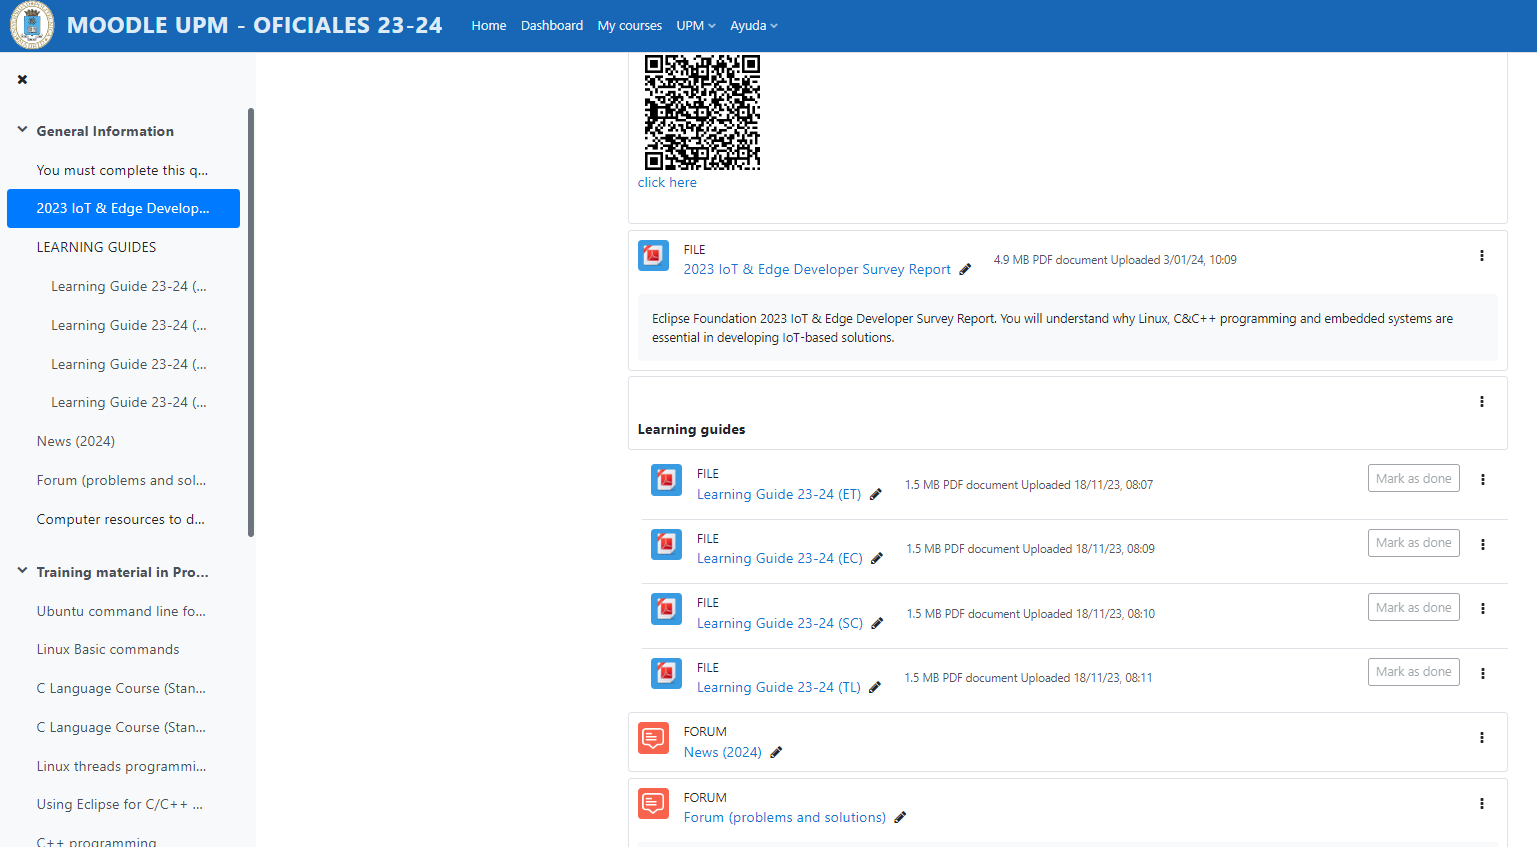
\includegraphics[scale=0.25]{trainingmaterials/presentation/schedule.png}
\end{frame}

\begin{frame}{Course assessment}
    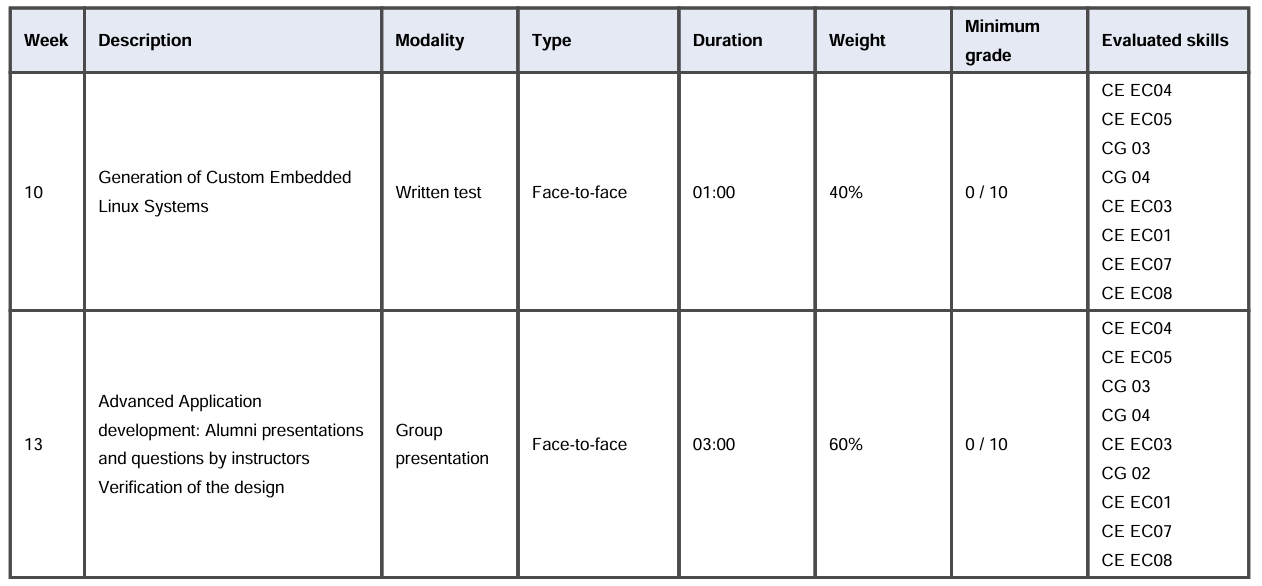
\includegraphics[scale=0.25]{trainingmaterials/presentation/assessment.png}
\end{frame}

% Resources Slide
\section{Resources}
\begin{frame}{Resources}
  \begin{itemize}
    \item \textbf{Equipment:}
    \begin{itemize}
      \item Raspberry Pi kit (board, charger, case, sensors, WiFi dongle).
      \item Desktop computer.
    \end{itemize}
    \item \textbf{Software:}
    \begin{itemize}
      \item Ubuntu, Buildroot, Raspbian, Eclipse.
    \end{itemize}
    \item \textbf{Moodle Platform:}
    \begin{itemize}
      \item Lecture slides
      \item Project documentation
      \item Additional reading materials
    \end{itemize}
  \end{itemize}
\end{frame}

\begin{frame}{Resources II}
    \begin{figure}[h]
        \centering
        \begin{subfigure}[b]{0.45\textwidth}
            \centering
            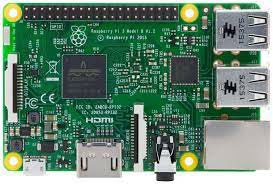
\includegraphics[width=\textwidth]{trainingmaterials/presentation/rpi.jpeg}
            \caption{RPI Board}
            \label{fig:rpi}
        \end{subfigure}
        \hfill
        \begin{subfigure}[b]{0.45\textwidth}
            \centering
            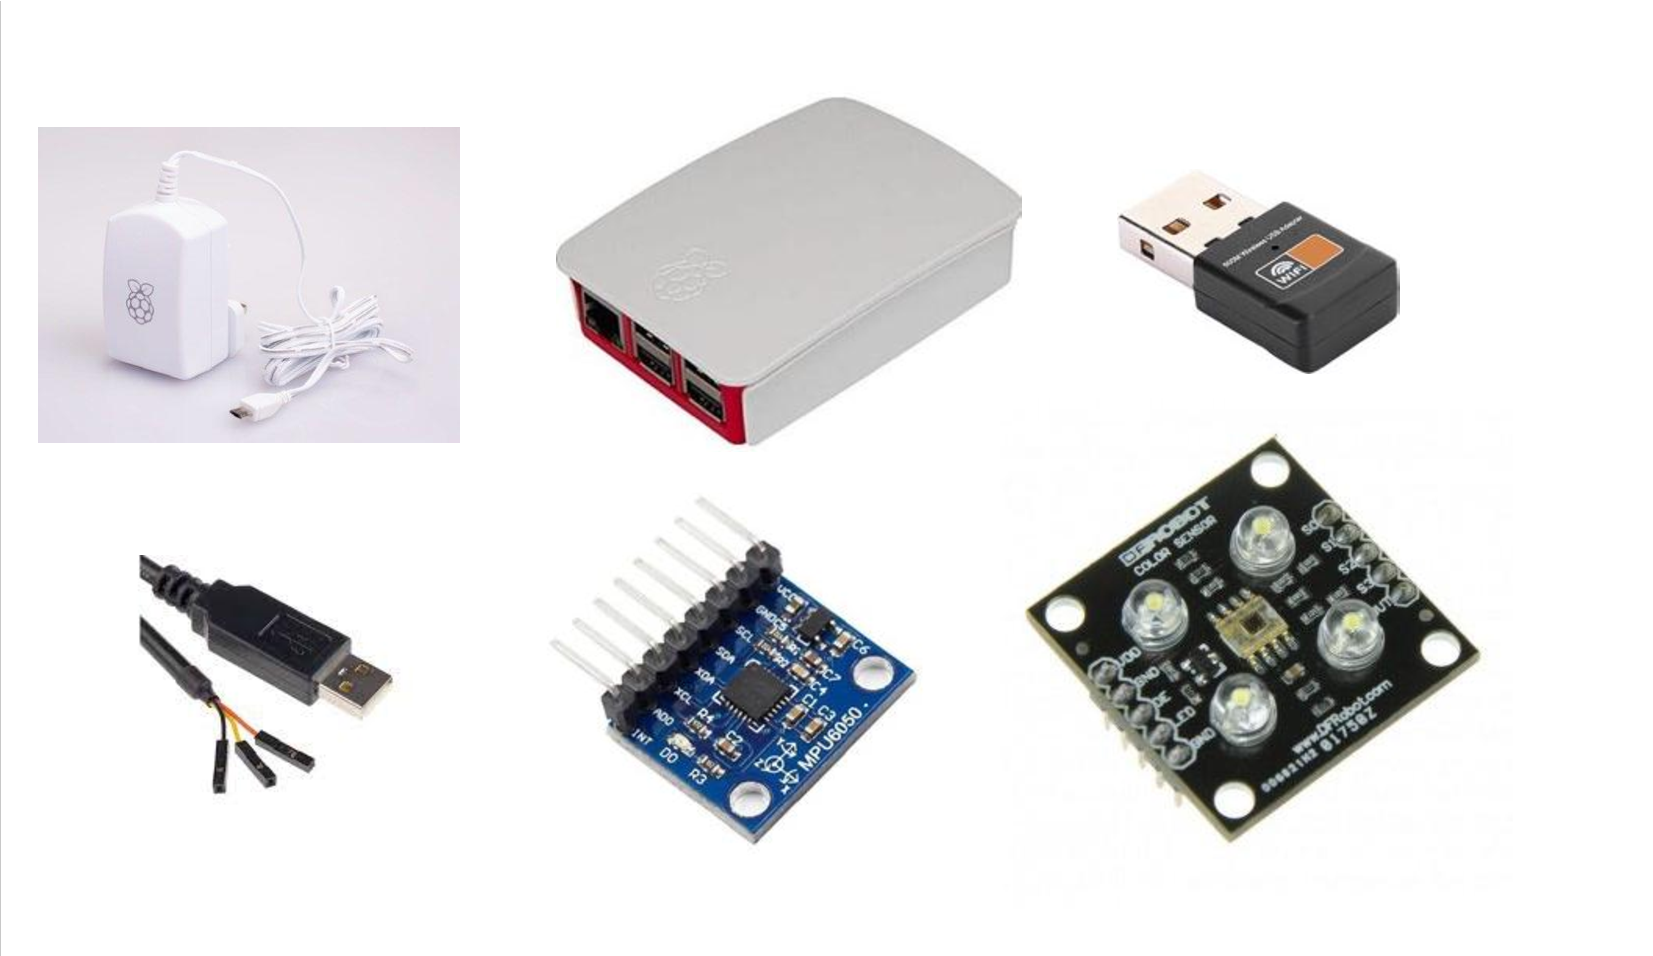
\includegraphics[width=\textwidth]{trainingmaterials/presentation/accesories.pdf}
            \caption{Accessories}
            \label{fig:accesories}
        \end{subfigure}
        \caption{Material on loan}
        \label{fig:figures}
    \end{figure}
\end{frame}

% References Slide
\begin{frame}{References}
  \begin{itemize}
    \item \textit{The Official Raspberry Pi Beginner’s Guide (5th Edition)} by Gareth Halfacree.
    \item \textit{Mastering Embedded Linux Programming (2nd Edition)} by Chris Simmonds.
    \item \textit{Pro Git (2nd Edition)} by Scott Chacon and Ben Straub.
    \item \textit{An Introduction to C \\ GUI Programming (2nd Edition)} by Simon Long.
  \end{itemize}
\end{frame}

\begin{frame}{Course Rules}
\begin{itemize}
    \item Use of mobile phones forbidden:
    \begin{itemize}
        \item Taking pictures
        \item Sending/receiving/checking messages from social networks and non-academic emails
    \end{itemize}
    \item Code authoring:
    \begin{itemize}
        \item You
        \item Adapted (state the lines that are copied and the changes you have made)
        \item Copied from the internet (add the source URL)
        \item Copied from your classmates (add their names)
    \end{itemize}
    \item Error reporting:
    \begin{itemize}
        \item Use Moodle, there is a specific forum for this
        \item Use correct (formal) language, respect the instructors and your classmates
        \item Provide enough information (and even files) to reproduce your problem
    \end{itemize}
\end{itemize}
\end{frame}